\chapter{Introducción}
\label{cap:intro}

Este manual acompaña al paquete de simulación \code{ball\_beam}, tercer experimento de la serie de sistemas de control tras el péndulo lineal~\cite{lineal} y el péndulo rotacional~\cite{rotacional}. Está organizado en dos partes:
\begin{itemize}
  \item \textbf{Parte teórica} (capítulos~\ref{cap:modelo}--\ref{cap:control}): modelo dinámico, análisis lineal, sensores y diseño de controladores.
  \item \textbf{Parte práctica} (capítulos~\ref{cap:simulink}--\ref{cap:practicas}): el modelo Simulink, la interfaz de código, la interfaz gráfica y una serie de prácticas guiadas.
\end{itemize}
La estructura, la convención de nombres y la interfaz son paralelas a las de los dos péndulos, de modo que lo aprendido allí se traslada casi sin cambios. Los resultados numéricos y todas las gráficas de este manual se han obtenido simulando el modelo Simulink del paquete (MATLAB R2025b) y se han contrastado con una réplica independiente en Python (apéndice~\ref{cap:validacion}).

\section{El sistema}

La \emph{bola y viga} es uno de los experimentos clásicos de los laboratorios de control~\cite{hauser1992}. Una bola de acero rueda por la ranura de una viga de \SI{42}{cm}. La viga pivota en su centro y la gira directamente el eje de salida de un motor de corriente continua con reductora (figura~\ref{fig:sistema}). Inclinando la viga, la gravedad empuja la bola hacia el extremo que queda más bajo; el objetivo es llevar la bola a una posición de referencia y mantenerla allí.

\begin{figure}[H]
\centering
% Esquema de la bola y viga (vista frontal)
\begin{tikzpicture}[>=Latex,scale=1.0,font=\small]
\def\al{12}            % ángulo dibujado [grados]
\def\Lh{4.2}           % semilongitud de la viga
\def\xb{2.2}           % posición de la bola a lo largo de la viga
% suelo y pedestal
\fill[gray!15] (-5.2,-2.6) rectangle (5.2,-2.4);
\draw[gray!60] (-5.2,-2.4) -- (5.2,-2.4);
\fill[gray!45] (-0.35,-2.4) rectangle (0.35,-0.3);
% motor (detrás del pivote)
\fill[c1!25,draw=c1!60!black] (0,0) circle (0.55);
\node[font=\scriptsize,c1!60!black] at (0,-0.95) {motor + reductora};
% eje horizontal de referencia
\draw[gray,dashed] (-\Lh-0.3,0) -- (\Lh+0.6,0);
% viga girada
\begin{scope}[rotate=\al]
  \fill[c2!20,draw=c2!70!black,thick] (-\Lh,-0.12) rectangle (\Lh,0.12);
  \fill[c2!60!black] (-\Lh-0.12,-0.12) rectangle (-\Lh,0.45);
  \fill[c2!60!black] (\Lh,-0.12) rectangle (\Lh+0.12,0.45);
  % bola
  \shade[ball color=gray!55] (\xb,0.47) circle (0.35);
  \draw[gray!50!black] (\xb,0.47) circle (0.35);
  % coordenada x
  \draw[|->,c4,thick] (0,-0.55) -- node[below,sloped]{$x$} (\xb,-0.55);
  \draw[c4,densely dotted] (\xb,-0.6) -- (\xb,0.12);
  % fuerza de la gravedad proyectada
  \draw[->,c5!60!black,thick] (\xb,0.47) -- ++(-1.1,0) node[above,font=\scriptsize]{$m g\sin\alpha$};
\end{scope}
\fill (0,0) circle (0.07);
% ángulo
\draw[->,thick] (2.9,0) arc[start angle=0,end angle=\al,radius=2.9] node[midway,right]{$\alpha$};
% peso
\draw[->,c5!60!black,thick] ({\xb*cos(\al)-0.47*sin(\al)},{\xb*sin(\al)+0.47*cos(\al)}) -- ++(0,-1.0) node[right,font=\scriptsize]{$mg$};
% tensión
\node[draw,fill=yellow!20,font=\scriptsize,align=center] (amp) at (-3.6,-1.5) {amplificador\\$\pm\SI{10}{V}$};
\draw[->,thick] (amp.east) -- node[above,font=\scriptsize]{$V$} (-0.6,-0.3);
% sensores
\node[font=\scriptsize,align=left,anchor=west] at (2.3,-1.7) {$x$: pista resistiva\\$\alpha$: encoder};
\end{tikzpicture}

\caption{Bola y viga. El motor inclina la viga un ángulo $\alpha$; la componente del peso a lo largo de la viga acelera la bola, cuya posición $x$ se mide desde el pivote.}
\label{fig:sistema}
\end{figure}

Frente a los péndulos hay tres diferencias importantes:
\begin{enumerate}
  \item \textbf{La inestabilidad nace de un doble integrador}: con la viga fija y horizontal la bola está en equilibrio indiferente, y cualquier inclinación la acelera sin límite. Con la viga libre la situación empeora: el peso de la bola inclina la viga hacia su lado (como un balancín), lo que acelera aún más la bola. El resultado es un polo real inestable que no existe en el modelo de libro de texto $\ddot x=-\tfrac57g\alpha$.
  \item \textbf{La estructura es en cascada}: el motor mueve la viga y la viga mueve la bola. Esto invita a un diseño en dos lazos anidados (un lazo rápido del ángulo de la viga y uno lento de la posición de la bola), alternativa natural al LQR.
  \item \textbf{La carga varía con el estado}: el peso de la bola ejerce sobre la viga un par $m g x$ que el motor debe compensar. Si no se tiene en cuenta, deja un error en régimen permanente.
\end{enumerate}

Se miden la posición de la bola, con una pista resistiva leída por un convertidor de 12 bits, y el ángulo de la viga, con un encoder en el eje de salida. Las velocidades las estima el controlador.

\begin{table}[H]
\centering\small
\begin{tabular}{@{}lll@{}}
\toprule
Símbolo & Significado & Convenio\\
\midrule
$x$ & posición de la bola [m] & $0$ = pivote; positiva hacia el extremo derecho; topes en $\pm\SI{19.7}{cm}$\\
$\alpha$ & ángulo de la viga [rad] & $0$ = horizontal; $\alpha>0$ \textbf{levanta} el extremo $+x$ (la bola rueda hacia $-x$)\\
$V$ & tensión del motor [V] & $V>0$ aumenta $\alpha$; saturación $\pm\SI{10}{V}$; topes de la viga en $\pm20^\circ$\\
$\vect s$ & estado & $[x,\ \xd,\ \alpha,\ \ald]^\top$\\
\bottomrule
\end{tabular}
\caption{Variables y convenio de signos.}
\label{tab:convenio}
\end{table}

\begin{nota}
La interfaz de código trabaja en \textbf{metros y radianes}. La interfaz gráfica y los campos \code{*\_cm} y \code{*\_deg} de los resultados (\code{x\_cm}, \code{r\_cm}, \code{al\_deg}, \code{alr\_deg}) usan centímetros y grados.
\end{nota}

\section{Contenido del paquete}

\begin{table}[H]
\centering\small
\begin{tabularx}{\linewidth}{@{}lX@{}}
\toprule
Archivo & Contenido\\
\midrule
\code{bb\_params.m} & Parámetros físicos, del motor, de los sensores y de los controladores.\\
\code{bb\_derived.m}, \code{bb\_linearize.m}, \code{bb\_lqr.m}, \code{bb\_design.m} & Magnitudes derivadas, linealización, LQR (con o sin toolbox) y cálculo de ganancias.\\
\code{bb\_plant\_block.m} & Dinámica no lineal con motor y topes (código del bloque \emph{MATLAB Function} de la planta).\\
\code{bb\_controller\_block.m} & Controlador discreto con 4 modos (código del bloque del controlador).\\
\code{bb\_ref\_block.m} & Generador de referencias de la bola.\\
\code{bb\_build\_model.m} & Genera el modelo \code{ballbeam\_sim.slx} mediante un script.\\
\code{BallBeam.m} & Clase con la interfaz de código: ensayos por lotes y control en vivo.\\
\code{bb\_gui.m} & Interfaz gráfica en vivo con animación 3D.\\
\code{bb\_draw.m}, \code{bb\_view.m}, \code{bb\_animate.m}, \code{bb\_plot\_results.m} & Escena 3D, puntos de vista, reproducción de ensayos y gráficas.\\
\code{examples.m} & Recorrido guiado por secciones.\\
\code{python\_reference\_sim.py} & Réplica independiente en Python usada para validar el modelo.\\
\code{validation/} & Scripts de validación cruzada Simulink--Python (apéndice~\ref{cap:validacion}).\\
\bottomrule
\end{tabularx}
\caption{Archivos del paquete \code{ball\_beam}.}
\label{tab:archivos}
\end{table}

\section{Requisitos y puesta en marcha}

Se necesita MATLAB y Simulink R2020b o posterior (se ha probado con R2025b). La Control System Toolbox es opcional: si no está instalada, \code{bb\_lqr} resuelve la ecuación de Riccati por el método del Hamiltoniano, igual que en los péndulos.

\begin{lstlisting}[caption={Primeros pasos.}]
cd src/ball_beam
bb_build_model                 % crea ballbeam_sim.slx (solo la primera vez)
bb_gui                         % interfaz gráfica en vivo
% o desde código:
bb = BallBeam();
bb.setInitialState([0.1 0 0 0]);   % bola a 10 cm, viga horizontal
bb.setMode('lqr');
res = bb.run(5);
bb_plot_results(res); bb.animate(res);
\end{lstlisting}

La figura~\ref{fig:frames} muestra la animación de un ensayo con el LQR: la referencia salta a \SI{12}{cm} y el controlador inclina primero la viga hacia abajo por el lado de la referencia para arrancar la bola, después la inclina al revés para frenarla y finalmente la deja casi horizontal.

\begin{figure}[H]
\centering
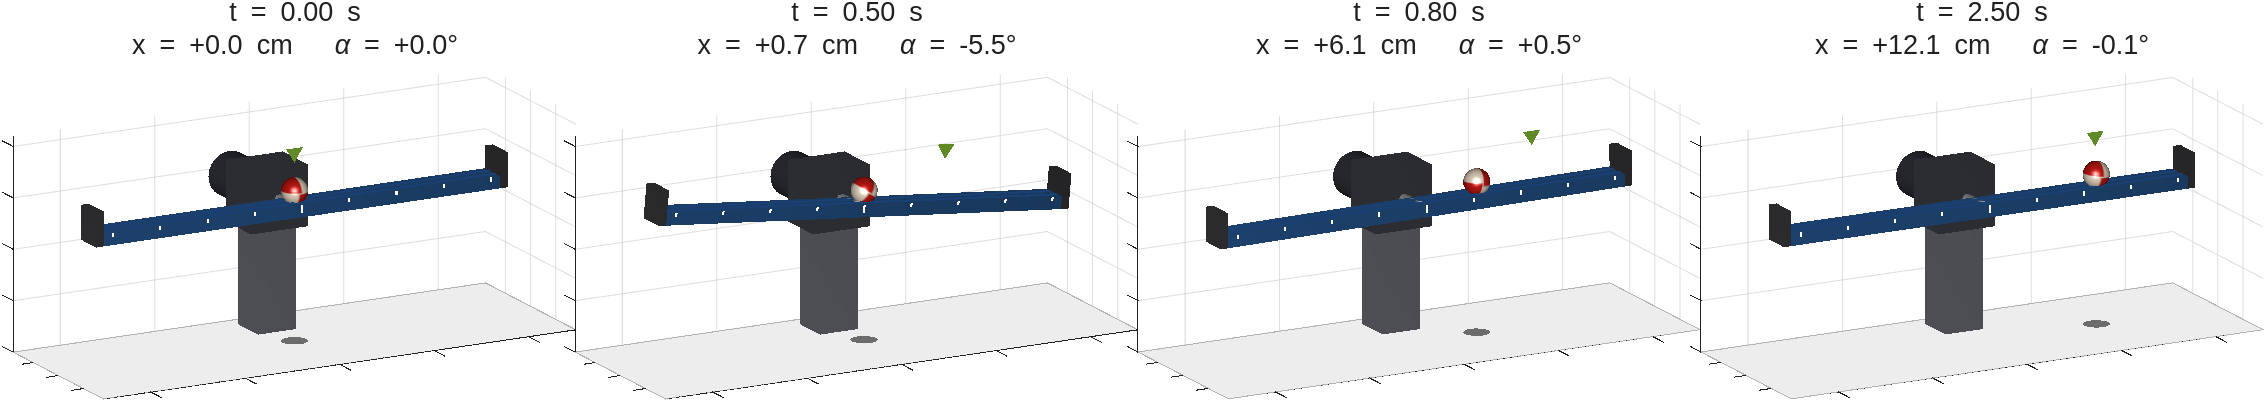
\includegraphics[width=\linewidth]{data/frames.png}
\caption{Fotogramas de la animación 3D (\code{bb\_animate}) durante un escalón de la referencia a \SI{12}{cm}. La bola tiene dos colores para que se vea girar; el triángulo verde marca la referencia.}
\label{fig:frames}
\end{figure}
